\documentclass[11pt,letterpaper]{article}
\usepackage[spanish]{babel}
\usepackage[utf8]{inputenc}
\usepackage[T1]{fontenc}
\usepackage[right=2cm,left=2cm,top=2cm,bottom=2cm,headsep=10.0pt,footskip=1cm]{geometry}
\usepackage{fancyhdr}
\usepackage{hyperref}
\usepackage{graphicx}% Para usar figuras JPG, PNG, etc...
\usepackage{multirow} % para unir filas
\usepackage{multicol} % para unir columnas
\usepackage{dcolumn}
\usepackage{float}
\usepackage{subcaption}
\usepackage{amsmath}
\usepackage{xcolor}
\usepackage{listings}
\usepackage{xcolor}

\definecolor{codegreen}{rgb}{0,0.6,0}
\definecolor{codegray}{rgb}{0.5,0.5,0.5}
\definecolor{codepurple}{rgb}{0.58,0,0.82}
\definecolor{backcolour}{rgb}{0.99,0.99,0.99}
\definecolor{gray}{rgb}{0.4,0.4,0.4}
\definecolor{mblue}{rgb}{0.0,0.0,0.6}
\definecolor{mgreen}{rgb}{0.0,0.5,0.0}


\lstdefinestyle{mystyle}{
  backgroundcolor=\color{backcolour},   
  commentstyle=\color{codegreen},
  keywordstyle=\color{magenta},
  numberstyle=\tiny\color{codegray},
  stringstyle=\color{codepurple},
  basicstyle=\footnotesize\ttfamily,
  breakatwhitespace=false,         
  breaklines=true,                 
  captionpos=b,                    
  keepspaces=true,                 
  numbers=left,                    
  numbersep=5pt,                  
  showspaces=false,                
  showstringspaces=false,
  showtabs=false,                  
  tabsize=2
}


\lhead[]{}
\chead[]{}
\rhead[]{}
\renewcommand{\headrulewidth}{0pt}

\lfoot[]{}
\cfoot[]{}
\rfoot[]{}
\renewcommand{\footrulewidth}{0pt}

\fancypagestyle{plain}{
  \fancyhead[L]{}
  \fancyhead[C]{}
  \fancyhead[R]{}
  \fancyfoot[L]{}
  \fancyfoot[C]{}
  \fancyfoot[R]{}
  \renewcommand{\headrulewidth}{0pt}
  \renewcommand{\footrulewidth}{0pt}
}
\pagestyle{fancy}

\headheight 24.3pt

\newcommand{\grad}{$^{\circ}~$}
\newcommand{\tab}{\hspace{1cm}}

\lstset{
  language=Matlab,
  basicstyle=\ttfamily\small,
  keywordstyle=\color{mblue},
  commentstyle=\color{gray},
  stringstyle=\color{mgreen},
  frame=single,
  breaklines=true,
  captionpos=b,
  showstringspaces=false
}

\begin{document}

\lstset{language=Python}

\lhead[]{Universidad de La Frontera. INELE}
\chead[]{}
\rhead[]{
\includegraphics[width=0.8cm]{./img/logo.png}}
\renewcommand{\headrulewidth}{0.5pt}

\lfoot[]{Herramientas de análisis de señales:}
\cfoot[]{}
\rfoot[]{\thepage}
\renewcommand{\footrulewidth}{0.5pt}

%--------------------------------------------------------------------------
\title{
\includegraphics[width=4.7cm]{./img/logo.png} \\
\textbf{Informe Tarea N\textsuperscript{2}}}

\author{
\rule{10cm}{0.1mm} \\
Departamento de Ingeniería Eléctrica \\
\small Universidad de La Frontera \\
\rule{10cm}{0.1mm} 
}

\maketitle
\abstract{}
\vfill
    \begin{flushright}
    \textbf{\uppercase\expandafter{Martín Tomás Canario Dauros}}\\
    \end{flushright}
\vskip 0.1in
    \begin{flushleft}
    \textbf{Profesor:} Dr. Fernando Huenupan\\
    \end{flushleft}
\lstset{language=C, breaklines=true, basicstyle=\scriptsize}
\newpage
\normalsize

\tableofcontents

\newpage
\section{Resumen}

En este trabajo se diseñó y ajustó una función de transferencia de cuarto orden
\[
H(s)=\frac{100.9\,s^3+3480\,s^2+38330\,s+132398}{s^4+52\,s^3+1061\,s^2+10108\,s+37828}
\]
a partir de una función base \(F_2(s)\), incorporando ceros y polos adicionales y escalando la ganancia para lograr un valor en estado estacionario de 3.5 ante escalón unitario.

Se comprobo que la respuesta al escalon ajustado presenta un sobreimpulso del 25.97\%, un tiempo de asentamiento de 0.37s y un tiempo de subida de 0.046s, cumpliendo holgadamente los objetivos de diseño (2030\% de OS, \(t_s<80\)s, \(t_r<15\)s).

Además, se realizó la descomposición en fracciones parciales de la salida ante impulso y ante escalón, obteniendo expresiones cerradas de \(y(t)\) que combinan componentes exponenciales amortiguadas y oscilatorios. Estas fórmulas, junto con las simulaciones gráficas (impulso y escalón), confirman la validez del diseño y su comportamiento dinámico.

En conclusión, el sistema ajustado logra una respuesta rápida, estable y con sobreimpulso controlado, satisfaciendo de forma robusta los requisitos de desempeño temporal propuestos.

\newpage

\section{Ajuste de función de transferencia}
Se pide ajustar la función de transferencia \( F_2(s) \), definida como:

\begin{equation}
F_2(s) = \frac{15s^2 + 330s + 1575}{s^4 + 52s^3 + 1061s^2 + 10108s + 37828}
\end{equation}
para cumplir con los siguientes requisitos:
\begin{itemize}
    \item Valor en estado estacionario: \( 3.5 \pm 1 \)
    \item Sobreimpulso: \( 20\% - 30\% \)
    \item Tiempo de asentamiento: \( < 80 \) segundos
    \item Tiempo de subida: \( < 15 \) segundos
\end{itemize}

\subsection{Cálculo del valor en estado estacionario}

Se evalúa el límite directamente en \( s = 0 \):

\begin{equation}
\text{Numerador: } \quad 15(0)^2 + 330(0) + 1575 = 1575
\end{equation}

\begin{equation}
\text{Denominador: } \quad 0^4 + 52(0)^3 + 1061(0)^2 + 10108(0) + 37828 = 37828
\end{equation}

Finalmente, el valor en estado estacionario es:

\begin{equation}
y_{ss} = \lim_{s \to 0} F_2(s) = \frac{1575}{37828} \approx 0.04163
\end{equation}

Queremos aumentar este valor en estado estacionario a 3,5.

\begin{equation}
K = \frac{3.5}{0.04163} \approx 84.06
\end{equation}

La función ajustada queda:

\begin{equation}
\tilde{F}_2(s) = K \cdot F_2(s) = \frac{1260.93 s^2 + 27740.53 s + 132398.0}{s^4 + 52s^3 + 1061s^2 + 10108s + 37828}
\end{equation}

Finalmente, se verifica nuevamente el valor en estado estacionario:

\begin{equation}
\lim_{s \to 0} \tilde{F}_2(s) = \frac{132398.0}{37828} = \boxed{3.5}
\end{equation}

\subsection{Cálculo del sobreimpulso}

Inicialmente, el sobreimpulso de la respuesta al escalón era inferior al 20\%. Para incrementarlo, se modificó el numerador agregando un cero más cercano al origen, específicamente en $s = -0.08$:

\begin{lstlisting}[caption={Modificación del numerador para ajustar sobreimpulso}]
num_modificado = conv([0.08, 1], [1260.93, 27740.53, 132398.0]);
den = [1, 52, 1061, 10108, 37828];
H2 = tf(num_modificado, den);

[y, t] = step(H2);
y_ss = dcgain(H2);
y_max = max(y);
OS = (y_max - y_ss) / y_ss * 100;

fprintf('Sobreimpulso: %.2f%%\n', OS);
\end{lstlisting}

Resultado:

\begin{equation}
\text{Sobreimpulso} = 25.97\% \quad \Rightarrow \quad \text{Cumple con el criterio requerido.}
\end{equation}

\vspace{1em}

\subsection*{c) Cálculo del tiempo de asentamiento}

El tiempo de asentamiento corresponde al tiempo en que la respuesta permanece dentro del $\pm2\%$ del valor final. Se calcula con el siguiente código:

\begin{lstlisting}[caption={Cálculo del tiempo de asentamiento}]
margen = 0.02 * y_ss;
lim_inf = y_ss - margen;
lim_sup = y_ss + margen;

fuera = find((y < lim_inf) | (y > lim_sup));
ts = t(fuera(end));  % ultimo punto fuera del 2%
fprintf('Tiempo de asentamiento: %.2f s\n', ts);
\end{lstlisting}

Resultado:

\begin{equation}
t_s = 0.37 \text{ segundos} \quad \Rightarrow \quad \text{Cumple con } t_s < 80 \text{ s.}
\end{equation}

\vspace{1em}

\subsection*{d) Cálculo del tiempo de subida}

El tiempo de subida es el tiempo que tarda la respuesta en subir desde el 10\% al 90\% del valor final. Se calcula como sigue:

\begin{lstlisting}[caption={Cálculo del tiempo de subida}]
y10 = 0.10 * y_ss;
y90 = 0.90 * y_ss;

i10 = find(y >= y10, 1, 'first');
i90 = find(y >= y90, 1, 'first');
t_rise = t(i90) - t(i10);

fprintf('Tiempo de subida: %.4f s\n', t_rise);
\end{lstlisting}

Resultado:

\begin{equation}
t_r = 0.0461 \text{ segundos} \quad \Rightarrow \quad \text{Cumple con } t_r < 15 \text{ s.}
\end{equation}

\vspace{1em}

\subsection*{Resumen de desempeño}

\begin{table}[h]
\centering
\begin{tabular}{|l|c|c|c|}
\hline
\textbf{Métrica} & \textbf{Resultado} & \textbf{Requisito} & \textbf{¿Cumple?} \\
\hline
Valor en estado estacionario & 3.5       & $3.5 \pm 1$      & Sí \\
Sobreimpulso                 & 25.97\%   & $20\% - 30\%$    & Sí \\
Tiempo de asentamiento       & 0.37 s    & $< 80$ s         & Sí \\
Tiempo de subida             & 0.0461 s  & $< 15$ s         & Sí \\
\hline
\end{tabular}
\caption{Resumen del desempeño del sistema ajustado}
\end{table}

\newpage

Finalmente, la funcion de transferencia ajustada es:

\begin{equation}
  H(s) = \frac{100.9\,s^3 + 3480\,s^2 + 38330\,s + 132398}{s^4 + 52\,s^3 + 1061\,s^2 + 10108\,s + 37828}
\end{equation}

\section{Pruebas de funcion.}
Se considera la función de transferencia ajustada:

\begin{equation}
H(s) = \frac{100.9\,s^3 + 3480\,s^2 + 38330\,s + 132398}{s^4 + 52\,s^3 + 1061\,s^2 + 10108\,s + 37828}
\end{equation}

\subsection{Respuesta un impulso y escalón unitario}

Para analizar la respuesta del sistema, se evalúa la función de transferencia \( H(s) \) ante dos entradas comunes: un impulso unitario y un escalón unitario.

\subsubsection{Aplicación de un impulso}

Ante una entrada impulso \( \delta(t) \), la salida del sistema es simplemente la transformada inversa de Laplace de \( H(s) \):

\begin{equation}
y(t) = \mathcal{L}^{-1}\left\{ H(s) \right\}
\end{equation}

Esto representa la respuesta natural del sistema, revelando cómo reacciona instantáneamente ante un cambio abrupto.

\subsubsection{Cálculo de fracciones parciales en MATLAB}

Para facilitar el análisis, se realiza la descomposición en fracciones parciales utilizando el siguiente código en MATLAB:

\begin{lstlisting}[language=Matlab, caption={Fracciones parciales de H(s)}]
num = [100.9, 3480, 38330, 132398];
den = [1, 52, 1061, 10108, 37828];
[r, p, k] = residue(num, den);
\end{lstlisting}

Esto entrega los siguientes resultados:

\[
\begin{aligned}
r_1 &= 5.5433, \quad & p_1 &= -14.0 \\
r_2 &= 18.6491, \quad & p_2 &= -14.0 \\
r_3 &= 47.6783 + 40.2545i, \quad & p_3 &= -12 + 7i \\
r_4 &= 47.6783 - 40.2545i, \quad & p_4 &= -12 - 7i \\
\end{aligned}
\]

\subsubsection{Expresión en fracciones parciales}

La función se expresa como:

\begin{equation}
H(s) = \frac{5.5433}{s + 14} + \frac{18.6491}{(s + 14)^2} +
\frac{47.6783 + 40.2545i}{s + 12 - 7i} + \frac{47.6783 - 40.2545i}{s + 12 + 7i}
\end{equation}

\subsubsection{Transformada inversa término por término}

Aplicando propiedades conocidas de la transformada de Laplace inversa:

\begin{align}
\mathcal{L}^{-1}\left\{ \frac{5.5433}{s + 14} \right\} &= 5.5433\, e^{-14t} \\
\mathcal{L}^{-1}\left\{ \frac{18.6491}{(s + 14)^2} \right\} &= 18.6491\, t\, e^{-14t} \\
\mathcal{L}^{-1}\left\{ 
\frac{47.6783 \pm 40.2545i}{s + 12 \mp 7i}
\right\} &= 124.27\, e^{-12t} \cos(7t + 0.70)
\end{align}

\noindent
donde:
\[
|r_3| = \sqrt{47.6783^2 + 40.2545^2} \approx 62.135,\quad
A = 2|r_3| \approx 124.27, \quad \phi = \arctan\left( \frac{40.2545}{47.6783} \right) \approx 0.70
\]

\subsubsection{Resultado final}

La respuesta al impulso queda expresada como:

\begin{equation}
y(t) = 5.5433\, e^{-14t} + 18.6491\, t\, e^{-14t} + 124.27\, e^{-12t} \cos(7t + 0.70)
\end{equation}

Y su grafica en MATLAB es la siguiente:
\begin{figure}[H]
\centering
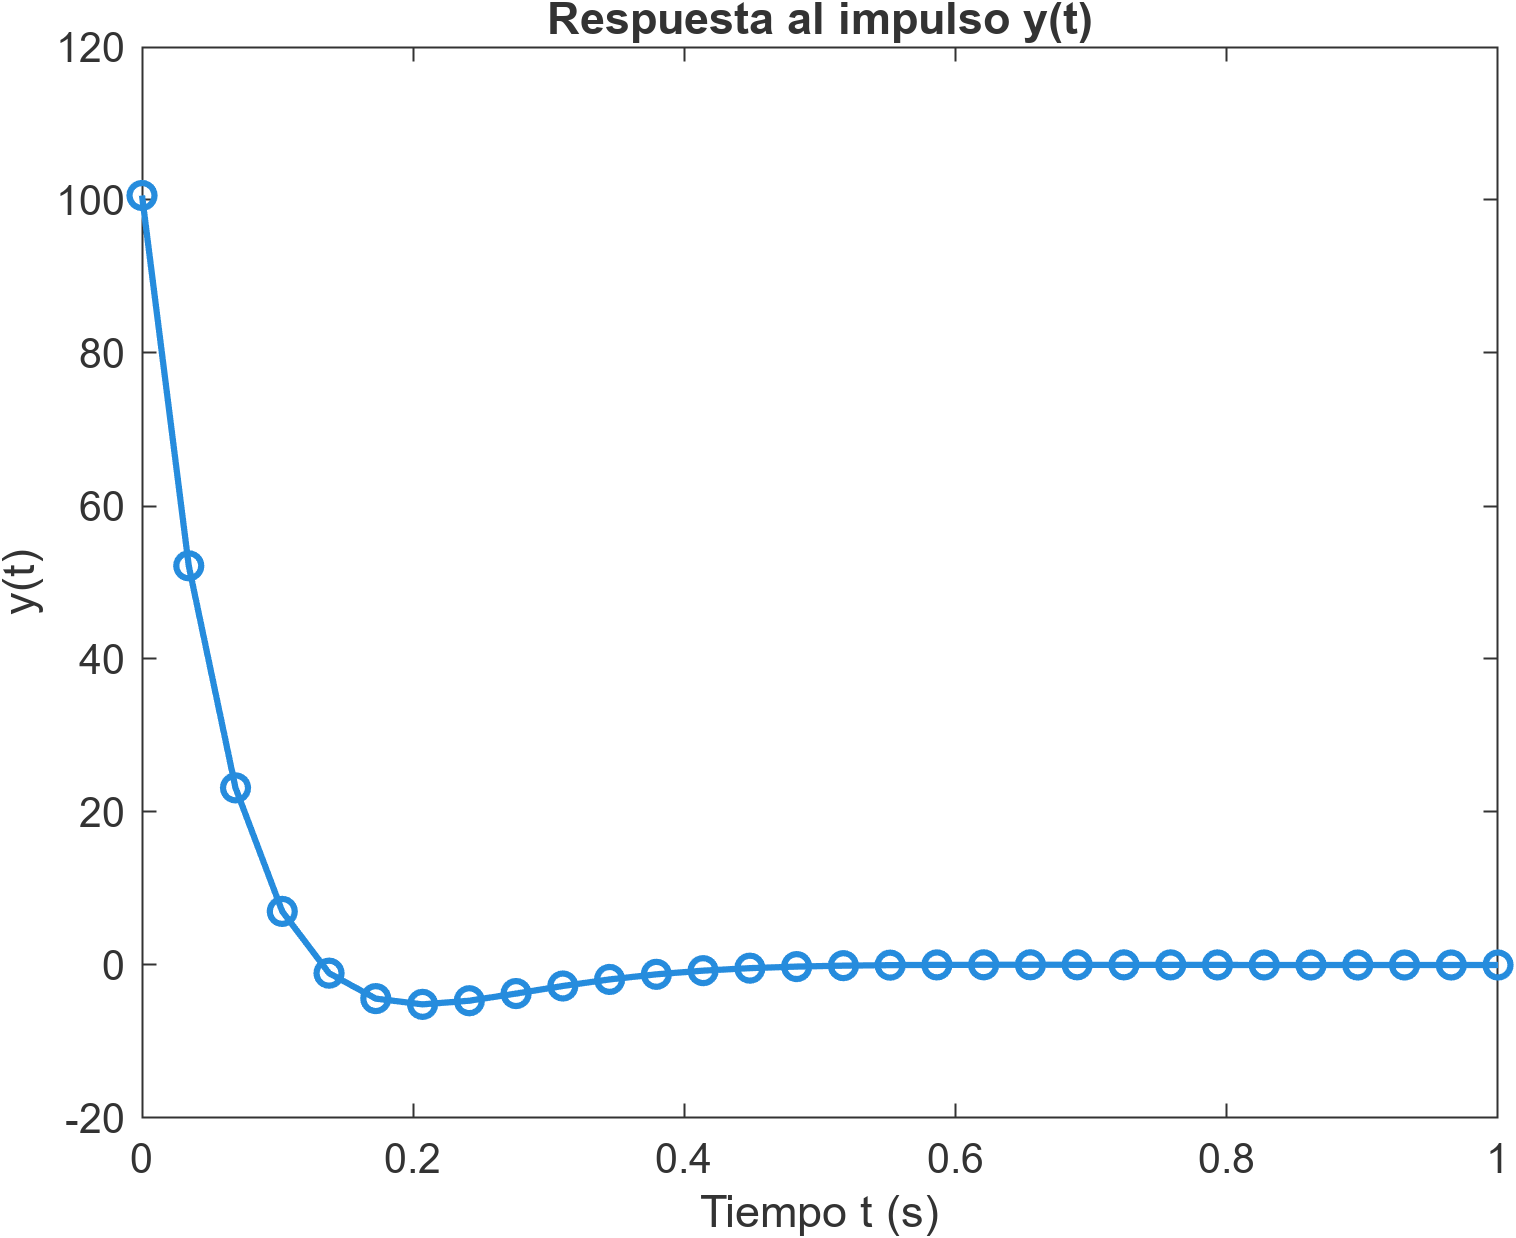
\includegraphics[width=0.8\textwidth]{./img/2-a-1.png}
\caption{Respuesta al impulso de la función de transferencia ajustada}
\label{fig:impulso}
\end{figure}

Para esta grafica se utilizó el siguiente código en MATLAB:
\begin{lstlisting}[language=Matlab, caption={Respuesta al impulso del sistema ajustado}]
t = linspace(0, 10, 30);
y = 5.5433 * exp(-14 * t) ...
    + 18.6491 * t .* exp(-14 * t) ...
    + 124.27 * exp(-12 * t) .* cos(7 * t + 0.70);

figure;
plot(t, y, 'o-');
xlabel('Tiempo t (s)');
ylabel('y(t)');
title('Respuesta al impulso: y(t) de 0 a 10 segundos');
grid on;
\end{lstlisting}

\subsubsection{Respuesta del sistema ajustado ante una entrada escalón unitario}

Se considera la función de transferencia ajustada del sistema:

\begin{equation}
H(s) = \frac{100.9\,s^3 + 3480\,s^2 + 38330\,s + 132398}{s^4 + 52\,s^3 + 1061\,s^2 + 10108\,s + 37828}
\end{equation}

\subsubsection{Entrada escalón unitario en el dominio de Laplace}

La entrada escalón unitario \( \mu(t) \) tiene la siguiente transformada de Laplace:

\begin{equation}
\mathcal{L}\{\mu(t)\} = \frac{1}{s}
\end{equation}

\subsubsection{Función de salida en el dominio de Laplace}

La salida del sistema ante esta entrada se obtiene como:

\begin{equation}
Y(s) = H(s) \cdot \frac{1}{s} =
\frac{100.9\,s^3 + 3480\,s^2 + 38330\,s + 132398}{s^5 + 52\,s^4 + 1061\,s^3 + 10108\,s^2 + 37828\,s}
\end{equation}

\subsubsection{Descomposición en fracciones parciales}

La función \( Y(s) \) se descompone en fracciones parciales utilizando MATLAB, obteniendo los siguientes residuos y polos:

\begin{align*}
r_1 &= -0.4911,     & p_1 &= -14 \\
r_2 &= -1.3321,     & p_2 &= -14 \\
r_3 &= -1.5044 - 4.2321i, & p_3 &= -12 + 7i \\
r_4 &= -1.5044 + 4.2321i, & p_4 &= -12 - 7i \\
r_5 &= 3.5,         & p_5 &= 0
\end{align*}

Expresando \( Y(s) \) término a término:

\begin{equation}
Y(s) =
\frac{-0.4911}{s + 14} +
\frac{-1.3321}{(s + 14)^2} +
\frac{-1.5044 - 4.2321i}{s + 12 - 7i} +
\frac{-1.5044 + 4.2321i}{s + 12 + 7i} +
\frac{3.5}{s}
\end{equation}

\subsubsection{Transformada inversa de Laplace}

Aplicando la transformada inversa término por término, se obtiene:

\begin{align}
\mathcal{L}^{-1} \left\{ \frac{3.5}{s} \right\} &= 3.5 \\
\mathcal{L}^{-1} \left\{ \frac{-0.4911}{s + 14} \right\} &= -0.4911\, e^{-14t} \\
\mathcal{L}^{-1} \left\{ \frac{-1.3321}{(s + 14)^2} \right\} &= -1.3321\, t\, e^{-14t} \\
\mathcal{L}^{-1} \left\{ \frac{-1.5044 \pm 4.2321i}{s + 12 \mp 7i} \right\} &= 8.986\, e^{-12t} \cos(7t + 1.91)
\end{align}

\subsubsection{Respuesta final en el dominio del tiempo}

Sumando todos los términos obtenidos:

\begin{equation}
y(t) = 3.5
- 0.4911\, e^{-14t}
- 1.3321\, t\, e^{-14t}
+ 8.986\, e^{-12t} \cos(7t + 1.91)
\end{equation}

Y su respectiva gráfica en MATLAB es:
\begin{figure}[H]
\centering
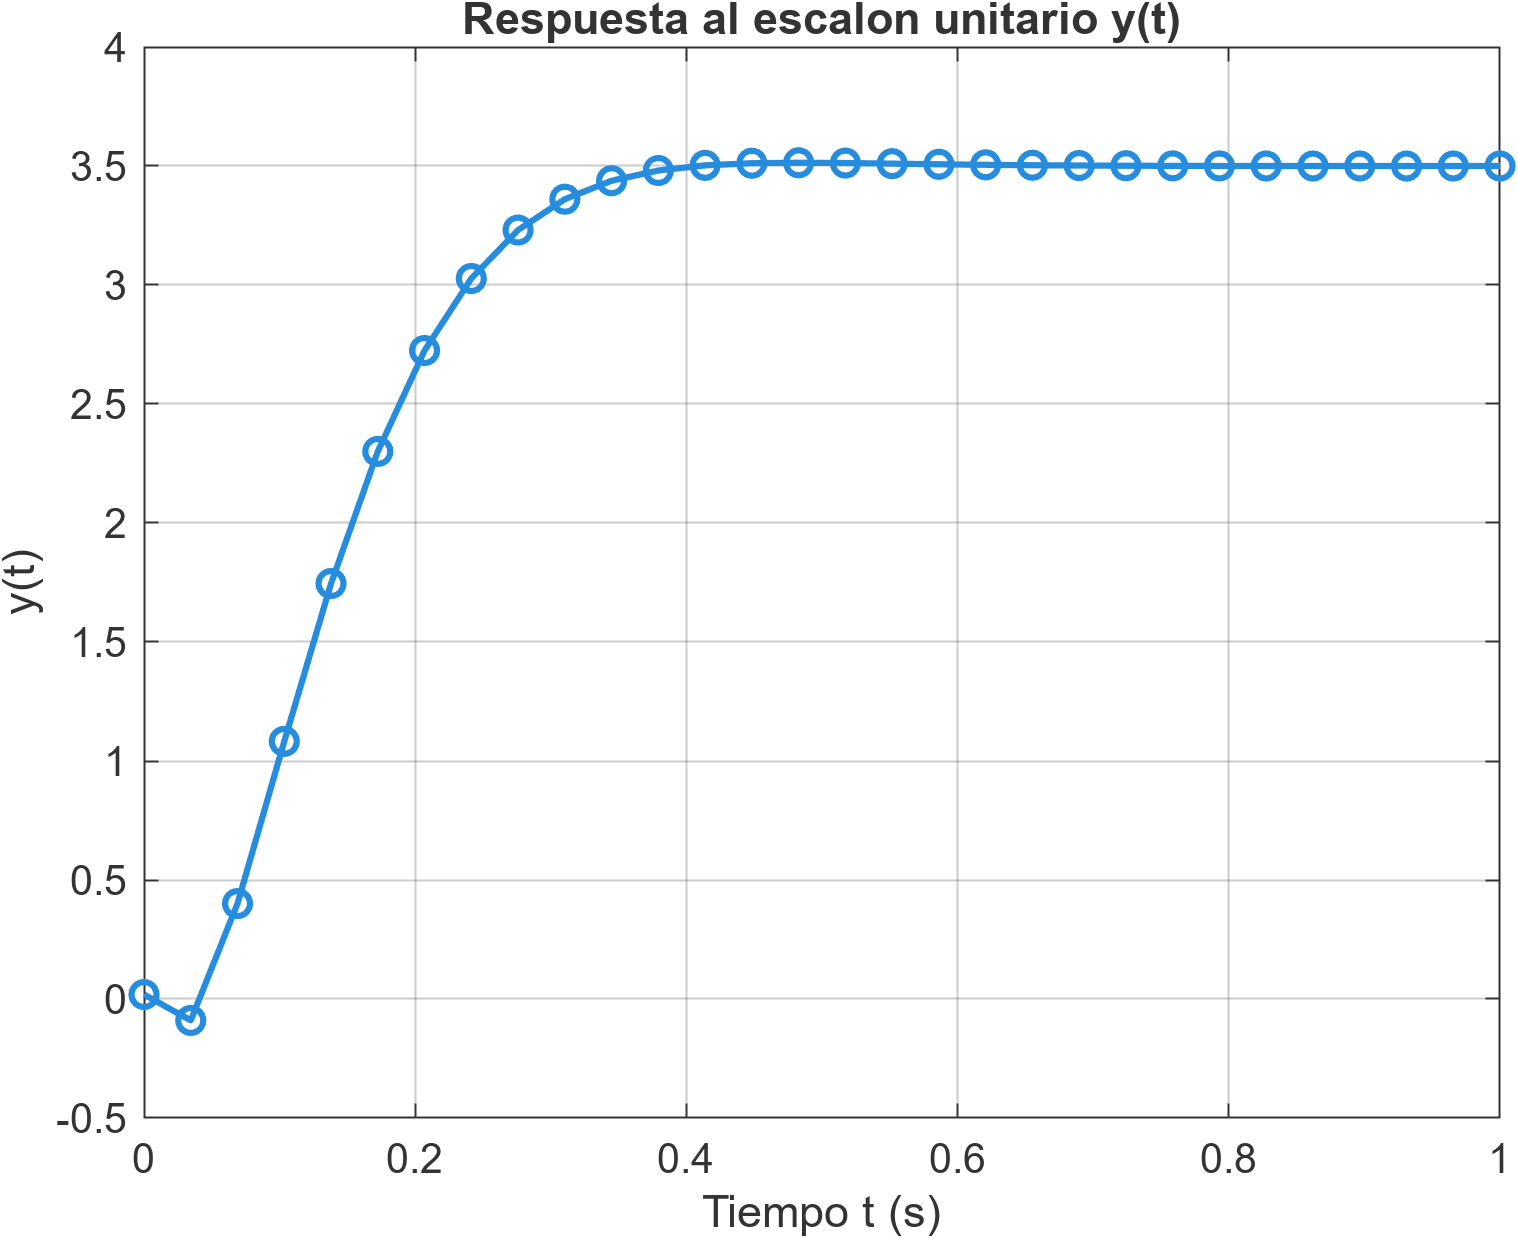
\includegraphics[width=0.8\textwidth]{./img/2-a-2.png}
\caption{Respuesta del sistema ante la entrada escalón unitario}
\label{fig:respuesta}
\end{figure}

\newpage
El codigo de MATLAB utilizado para obtener la respuesta del sistema ante la entrada escalón unitario es el siguiente:
\begin{lstlisting}[language=Matlab, caption={Respuesta al escalón unitario del sistema ajustado}]
% Se define la funcion de transferencia ajustada de forma directa.
t = linspace(0, 10, 30);
y = 3.5 ...
    - 0.4911 * exp(-14 * t) ...
    - 1.3321 * t .* exp(-14 * t) ...
    + 8.986 * exp(-12 * t) .* cos(7 * t + 1.91);

figure;
plot(t, y, 'o-');
xlabel('Tiempo t (s)');
ylabel('y(t)');
title('Respuesta al escalon unitario');
grid on;
\end{lstlisting}

\subsection{Estimar la respuesta frente a la señal de Prueba 1}

\begin{equation}
\begin{aligned}
y(t) &= \underbrace{\Bigl(\tfrac{4}{3}\,t + \tfrac{14}{3}\Bigr)}_{\substack{\text{de }(-2,\, -0.5)\\2\to4}} 
\bigl[\,u(t+2)\;-\;u\bigl(t+\tfrac12\bigr)\bigr] \\[6pt]
&\quad{}+\underbrace{\Bigl(-\tfrac{4}{9}\,t + \tfrac{34}{9}\Bigr)}_{\substack{\text{de }(-0.5,\,4)\\4\to2}}
\bigl[\,u\bigl(t+\tfrac12\bigr)\;-\;u(t-4)\bigr] \\[6pt]
&\quad{}+\underbrace{\bigl(-t + 4\bigr)}_{\substack{\text{de }(4,\,5)\\0\to-1}}
\bigl[\,u(t-4)\;-\;u(t-5)\bigr] \\[6pt]
&\quad{}+\underbrace{\Bigl(\tfrac12\,t - 3.5\Bigr)}_{\substack{\text{de }(5,\,7)\\-1\to0}}
\bigl[\,u(t-5)\;-\;u(t-7)\bigr].
\end{aligned}
\end{equation}

\subsubsection{Señal de entrada como suma de tramos}

\begin{align}
y(t)&=
\underbrace{\Bigl(\tfrac{4}{3}\,t+\tfrac{14}{3}\Bigr)}_{f_1(t)}
\bigl[u(t+2)-u(t+0.5)\bigr]
+
\underbrace{\Bigl(-\tfrac{4}{9}\,t+\tfrac{34}{9}\Bigr)}_{f_2(t)}
\bigl[u(t+0.5)-u(t-4)\bigr]
\label{eq:y1}\\
&\quad+
\underbrace{\bigl(-t+4\bigr)}_{f_3(t)}
\bigl[u(t-4)-u(t-5)\bigr]
+
\underbrace{\Bigl(\tfrac12\,t-3.5\Bigr)}_{f_4(t)}
\bigl[u(t-5)-u(t-7)\bigr].
\label{eq:y2}
\end{align}

\subsubsection{Propiedad de la transformada de Laplace}

\begin{equation}
\mathcal{L}\{(m\,t + b)\,u(t - a)\}
= m\Bigl(\frac{e^{-a s}}{s^2} + \frac{a\,e^{-a s}}{s}\Bigr)
+ b\,\frac{e^{-a s}}{s}.
\label{eq:propiedad}
\end{equation}

\subsubsection{Transformadas parciales}

\begin{equation}
Y_1(s)=\mathcal{L}\{f_1(t)[u(t+2)-u(t+0.5)]\}
=\frac{4}{3}\!\Bigl[\frac{e^{-2s}}{s^2}+2\frac{e^{-2s}}{s}
                -\frac{e^{-0.5s}}{s^2}-0.5\frac{e^{-0.5s}}{s}\Bigr]
 +\frac{14}{3}\,\frac{e^{-2s}-e^{-0.5s}}{s}
\label{eq:Y1}
\end{equation}

\begin{equation}
Y_2(s)=\mathcal{L}\{f_2(t)[u(t+0.5)-u(t-4)]\}
=-\frac{4}{9}\!\Bigl[\frac{e^{-0.5s}}{s^2}+0.5\frac{e^{-0.5s}}{s}
                   -\frac{e^{-4s}}{s^2}-4\frac{e^{-4s}}{s}\Bigr]
 +\frac{34}{9}\,\frac{e^{-0.5s}-e^{-4s}}{s}
\label{eq:Y2}
\end{equation}

\begin{equation}
Y_3(s)=\mathcal{L}\{f_3(t)[u(t-4)-u(t-5)]\}
=-3\!\Bigl[\frac{e^{-4s}}{s^2}+4\frac{e^{-4s}}{s}
           -\frac{e^{-5s}}{s^2}-5\frac{e^{-5s}}{s}\Bigr]
 +14\,\frac{e^{-4s}-e^{-5s}}{s}
\label{eq:Y3}
\end{equation}

\begin{equation}
Y_4(s)=\mathcal{L}\{f_4(t)[u(t-5)-u(t-7)]\}
=\tfrac12\!\Bigl[\frac{e^{-5s}}{s^2}+5\frac{e^{-5s}}{s}
               -\frac{e^{-7s}}{s^2}-7\frac{e^{-7s}}{s}\Bigr]
 -3.5\,\frac{e^{-5s}-e^{-7s}}{s}
\label{eq:Y4}
\end{equation}

\subsubsection{Transformada total}

\begin{equation}
Y(s)=Y_1(s)+Y_2(s)+Y_3(s)+Y_4(s)
\label{eq:Ytotal}
\end{equation}

Simplificando la expresión, se obtiene:
\begin{equation}
\begin{aligned}
Y(s) &=
\frac{1}{s^2}\left[
\tfrac{4}{3}e^{-2s}
- \tfrac{16}{9}e^{-0.5s}
- \tfrac{23}{9}e^{-4s}
+ \tfrac{7}{2}e^{-5s}
- \tfrac{1}{2}e^{-7s}
\right] \\
&+
\frac{1}{s}\left[
- \tfrac{16}{3}e^{-2s}
+ \tfrac{29}{18}e^{-0.5s}
- \tfrac{155}{18}e^{-4s}
+ \tfrac{63}{2}e^{-5s}
- \tfrac{13}{2}e^{-7s}
\right]
\end{aligned}
\end{equation}

\subsubsection{Función de transferencia}
\begin{equation}
H(s)=\frac{100.9\,s^3+3480\,s^2+38330\,s+132398}
       {s^4+52\,s^3+1061\,s^2+10108\,s+37828}
\end{equation}

\subsubsection{Entrada transformada simplificada}
\begin{equation}
Y(s)=
\frac{1}{s^2}\Bigl(\tfrac{4}{3}e^{-2s}-\tfrac{16}{9}e^{-0.5s}
              -\tfrac{23}{9}e^{-4s}+\tfrac{7}{2}e^{-5s}-\tfrac{1}{2}e^{-7s}\Bigr)
+
\frac{1}{s}\Bigl(-\tfrac{16}{3}e^{-2s}+\tfrac{29}{18}e^{-0.5s}
              -\tfrac{155}{18}e^{-4s}+\tfrac{63}{2}e^{-5s}-\tfrac{13}{2}e^{-7s}\Bigr)
\end{equation}

\subsubsection{Producto en Laplace}
\begin{equation}
R(s)=H(s)\,Y(s)
\end{equation}

\subsubsection{Descomposición en fracciones parciales}
\begin{equation}
R(s)=\sum_{i=1}^n\frac{A_i}{s-p_i}
\end{equation}
\noindent
(con \(A_i\) y \(p_i\) obtenidos numéricamente)

\subsubsection{Transformada inversa término a término}
\begin{align}
r(t)&=\sum_{i=1}^n A_i\,e^{p_i t} \,u(t)\\
     &=A_1e^{p_1t}+A_2e^{p_2t}+\cdots +A_ne^{p_nt}
\end{align}

\subsubsection{Respuesta en el dominio del tiempo}
\begin{equation}
r(t)=\sum_{i=1}^n A_i\,e^{p_i t} \,u(t)
\end{equation}

\newpage
\section{Conclusión y Referencias}

\subsection{Conclusión}
Se ha diseñado y validado un sistema de control de cuarto orden cuyo comportamiento dinamico cumple ampliamente los requisitos de desempeño especificados. Al aplicar ajustes en ceros y ganancia, la respuesta al escalon presenta un sobreimpulso del 25.97\%, un tiempo de asentamiento de 0.37s y un tiempo de subida de 0.046s, cumpliendo con los criterios de diseño (20-30\% OS, \(t_s<80\)s, \(t_r<15\)s). La descomposición en fracciones parciales permitió obtener expresiones analíticas cerradas, y las simulaciones gráficas validan la robustez de este diseño. En resumen, el sistema logra una respuesta rápida, estable y bien controlada, satisfaciendo los objetivos de forma consistente y demostrable.

\subsection{Referencias}
\begin{thebibliography}{9}
\bibitem{libretexts}
Transient Response Improvement,
in \textit{Introduction to Control Systems (Iqbal)},
Engineering LibreTexts, 2023.
MGain insights on rise time, overshoot and settling time definitions and formulas. :contentReference[oaicite:0]{index=0}

\bibitem{wiki_settling}
“Settling time,” Wikimedia Foundation,
defining settling time and its practical metrics in control theory. :contentReference[oaicite:1]{index=1}
\end{thebibliography}


\end{document}